\documentclass[useAMS,usenatbib,a4paper,referee]{mn2e}

\pdfpagewidth=\paperwidth 
\pdfpageheight=\paperheight

\newcommand{\sub}[2]{\ensuremath{#1_{\mathrm{#2}}}}
\newcommand{\super}[2]{\ensuremath{#1^{\mathrm{#2}}}}
\newcommand{\rcore}{\sub{r}{core}}
\newcommand{\unit}[2]{\ensuremath{\textrm{#1}^{#2}}}

%\newcommand\aj{{AJ}}% 
          % Astronomical Journal 
\newcommand\araa{{ARA\&A}}% 
          % Annual Review of Astron and Astrophys 
\newcommand\apj{{ApJ}}% 
          % Astrophysical Journal 
\newcommand\apjl{{ApJ}}% 
          % Astrophysical Journal, Letters 
\newcommand\apjs{{ApJS}}% 
          % Astrophysical Journal, Supplement 
\newcommand\ao{{Appl.~Opt.}}% 
          % Applied Optics 
\newcommand\apss{{Ap\&SS}}% 
          % Astrophysics and Space Science 
\newcommand\aap{{A\&A}}% 
          % Astronomy and Astrophysics 
\newcommand\aapr{{A\&A~Rev.}}% 
          % Astronomy and Astrophysics Reviews 
\newcommand\aaps{{A\&AS}}% 
          % Astronomy and Astrophysics, Supplement 
\newcommand\azh{{AZh}}% 
          % Astronomicheskii Zhurnal 
\newcommand\baas{{BAAS}}% 
          % Bulletin of the AAS 
\newcommand{\jcap}{J. Cosm. Astropart. Phys.}
	% Journal of Cosmology and Astroparticle Physics
\newcommand\jrasc{{JRASC}}% 
          % Journal of the RAS of Canada 
\newcommand\memras{{MmRAS}}% 
          % Memoirs of the RAS 
\newcommand\mnras{{MNRAS}}% 
          % Monthly Notices of the RAS 
\newcommand\pra{{Phys.~Rev.~A}}% 
          % Physical Review A: General Physics 
\newcommand\prb{{Phys.~Rev.~B}}% 
          % Physical Review B: Solid State 
\newcommand\prc{{Phys.~Rev.~C}}% 
          % Physical Review C 
\newcommand\prd{{Phys.~Rev.~D}}% 
          % Physical Review D 
\newcommand\pre{{Phys.~Rev.~E}}% 
          % Physical Review E 
\newcommand\prl{{Phys.~Rev.~Lett.}}% 
          % Physical Review Letters 
\newcommand\pasp{{PASP}}% 
          % Publications of the ASP 
\newcommand\pasj{{PASJ}}% 
          % Publications of the ASJ 
\newcommand\qjras{{QJRAS}}% 
          % Quarterly Journal of the RAS 
\newcommand\skytel{{S\&T}}% 
          % Sky and Telescope 
\newcommand\solphys{{Sol.~Phys.}}% 
          % Solar Physics 
\newcommand\sovast{{Soviet~Ast.}}% 
          % Soviet Astronomy 
\newcommand\ssr{{Space~Sci.~Rev.}}% 
          % Space Science Reviews 
\newcommand\zap{{ZAp}}% 
          % Zeitschrift fuer Astrophysik 
\newcommand\nat{{Nature}}% 
          % Nature 
\newcommand\iaucirc{{IAU~Circ.}}% 
          % IAU Cirulars 
\newcommand\aplett{{Astrophys.~Lett.}}% 
          % Astrophysics Letters 
\newcommand\apspr{{Astrophys.~Space~Phys.~Res.}}% 
          % Astrophysics Space Physics Research 
\newcommand\bain{{Bull.~Astron.~Inst.~Netherlands}}% 
          % Bulletin Astronomical Institute of the Netherlands 
\newcommand\fcp{{Fund.~Cosmic~Phys.}}% 
          % Fundamental Cosmic Physics 
\newcommand\gca{{Geochim.~Cosmochim.~Acta}}% 
          % Geochimica Cosmochimica Acta 
\newcommand\grl{{Geophys.~Res.~Lett.}}% 
          % Geophysics Research Letters 
\newcommand\jcp{{J.~Chem.~Phys.}}% 
          % Journal of Chemical Physics 
\newcommand\jgr{{J.~Geophys.~Res.}}% 
          % Journal of Geophysics Research 
\newcommand\jqsrt{{J.~Quant.~Spec.~Radiat.~Transf.}}% 
          % Journal of Quantitiative Spectroscopy and Radiative Trasfer 
\newcommand\memsai{{Mem.~Soc.~Astron.~Italiana}}% 
          % Mem. Societa Astronomica Italiana 
\newcommand\nphysa{{Nucl.~Phys.~A}}% 
          % Nuclear Physics A 
\newcommand\physrep{{Phys.~Rep.}}% 
          % Physics Reports 
\newcommand\physscr{{Phys.~Scr}}% 
          % Physica Scripta 
\newcommand\planss{{Planet.~Space~Sci.}}% 
          % Planetary Space Science 
\newcommand\procspie{{Proc.~SPIE}}% 
          % Proceedings of the SPIE 
\let\astap=\aap 
\let\apjlett=\apjl 
\let\apjsupp=\apjs 
\let\applopt=\ao 


\bibliographystyle{astron}

\usepackage{graphicx} 
\usepackage{epstopdf} 
\usepackage{amsmath}
\usepackage{hyperref}

\begin{document}

\title{Action-space clustering of streams can be used to map the Galactic potential}
%authors in no particular order
\author[]{Robyn E. Sanderson, Amina Helmi${}^{1}$, David Hogg${}^{2}$\\
${}^{1}$Kapteyn Astronomical Institute, P.O. Box 800, 9700 AV Groningen, The Netherlands\\
${}^{2}$NYU}

\maketitle

\begin{abstract}
We use a simple example to demonstrate that, given a parameterized model of the Galactic potential, the set of parameters retrieved by maximizing the Kullback-Leibler divergence of a set of points clustered in action space are the input parameters. We further show that if a different parameterization is used for maximization than for the input, the parameters retrieved are the best-fit of the output potential to the input at the measured points. This method will allow us to capitalize on the existence of kinematic substructures in the Galaxy to measure the potential without explicity identifying streams.
\end{abstract}

%\begin{keywords}
%\end{keywords}

\section{About the Kullback-Liebler divergence}
\label{sec:kld}

The Kullback-Liebler divergence (KLD) is a way of comparing the degree of clustering (or amount of information) in two different statistical distributions. For a continuous random variable $\mathbf{x}$, the KLD \emph{from} distribution $p(\mathbf{x}$ \emph{to} distribution $q(\mathbf{x}$ is defined as
\begin{equation}
 D_{KL}(p\to q) \equiv \int p(\mathbf{x}) \log \frac{p(\mathbf{x})}{q(\mathbf{x})} d\mathbf{x}.
\end{equation}
The KLD is not symmetric; it can be considered a measure of the relative entropy between $p$ and $q$. The lower the entropy of $p$ relative to $q$, the higher the value of $D_{KL}$ (Figure \ref{fig:1Dexample}).
\begin{figure*}
 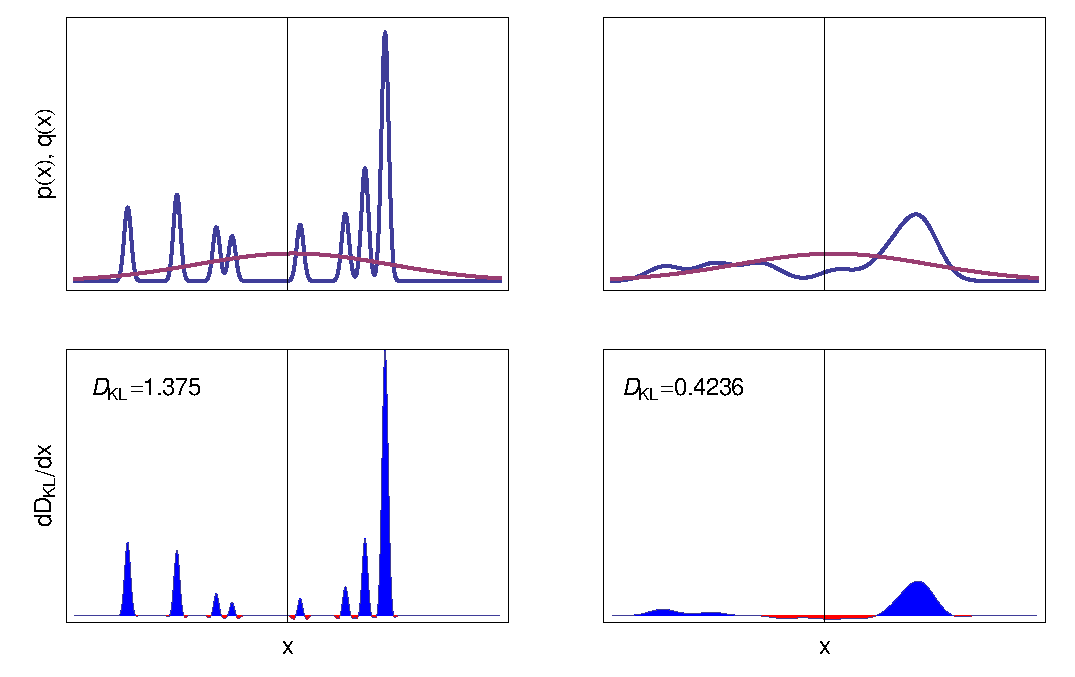
\includegraphics[width=0.95\textwidth]{KLDiv_1D_Example}
\caption{If the distribution $p$ (blue line) is much more clustered than distribution $q$ (pink line) as shown in the example on the left (upper panel), then the integrand (lower panel) is large and $D_{KL}$ is large. A distribution $p$ that is only somewhat less smooth than $q$ (right column) has a lower $D_{KL}$.}
\label{fig:1Dexample}
\end{figure*}

If a set of $N$ points $\mathbf{x}_i$ are independent random deviates drawn from $p$, then we can use them to do a Monte Carlo approximation to the integral:
\begin{equation}
  \tilde{D}_{KL}(p\to q) = \frac{1}{N} \sum_{i}^{N} \log \frac{p(\mathbf{x}_i)}{q(\mathbf{x}_i)}
\end{equation}
This works even if $p$ is not known. In that case you use the ``observed'' distribution $\tilde{p}$ constructed in some way from the observed $\mathbf{x}_i$ instead of the true distribution $p$. An example using the two distributions on the left of Figure \ref{fig:1Dexample} is shown in Figure \ref{fig:monteCarlo}.
\begin{figure*}
 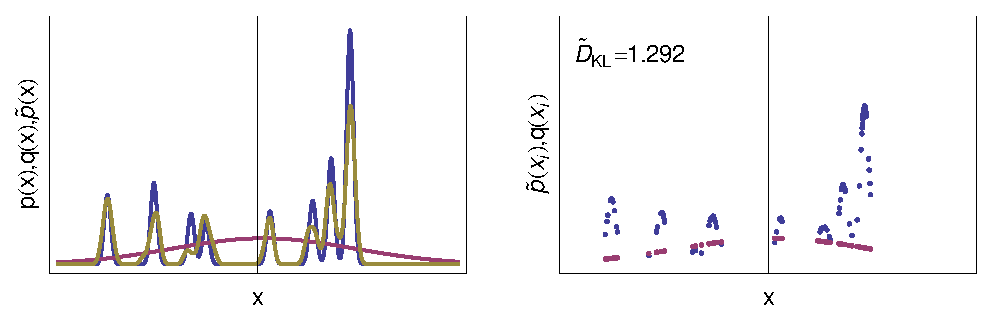
\includegraphics[width=0.95\textwidth]{monteCarlo}
\caption{Left panel: The observed distribution $\tilde{p}$ (yellow) can be constructed from the $\mathbf{x}_i$ (in this case using Gaussian smoothing) to approximate the true parent distribution $p$ (blue). Right panel: Both $\tilde{p}$ (blue) and $q$ (pink) are evaluated at the $\mathbf{x}_i$ to calculate the estimated KLD, $\tilde{D}_{KL}$. The value obtained is close to the one found using the exact parent distribution.}
\label{fig:monteCarlo}
\end{figure*}

Finally, since $p$ and $q$ are probability distributions, the KLD is invariant under transformations of $\mathbf{x}$ because $p(\mathbf{x}) d\mathbf{x} = p(\mathbf{y}) d\mathbf{y}$, for any continuously differentiable $\mathbf{y}(\mathbf{x})$:
\begin{equation}
  \int  \log \frac{p(\mathbf{x})}{q(\mathbf{x})} p(\mathbf{x}) d\mathbf{x} = \int \log \frac{p(\mathbf{y}) d\mathbf{y}/d\mathbf{x}}{q(\mathbf{y})d\mathbf{y}/d\mathbf{x}} p(\mathbf{y}) d\mathbf{y} =  \int  \log \frac{p(\mathbf{y})}{q(\mathbf{y})} p(\mathbf{y}) d\mathbf{y} 
\end{equation}


The KLD is a promising tool for using stellar streams to constrain the Galactic potential. The clustering of streams in action space is assumed to be tightest when the correct potential (or the closest one to the real potential) is used to compute the actions. So if we take the actions $\mathbf{I}$ as the random variable, we can compare the observed distribution $\tilde{O}(\mathbf{I}|\mathbf{a})$ obtained by computing the values $\mathbf{I}_i$ for a given set of potential parameters $\mathbf{a}$ to a smooth distribution $T$ that fits the same actions (for example the Gaussian with mean and width equal to the mean and standard deviation of the $\mathbf{I}_i$) using the Monte-Carlo form $\tilde{D}_{KL}$:
\begin{equation}
\sub{\tilde{D}}{KL} \equiv \sum_i^{N_*} \log \frac{O[\mathbf{I}_i(\mathbf{a})|\mathbf{a}]}{T[\mathbf{I}_i(\mathbf{a})|\mathbf{a}]}
\end{equation}
As the parameters approach the best-fit potential, the value of $\tilde{D}_{KL}$ will increase as the actions of stars in the various streams cluster more tightly together. 

The KLD is invariant under parameter transformations, but we've also collapsed it to 3D from 6D by only considering the actions. So somehow we have to account for $\mathbf{a}$-dependence if we try to transform back to observables. We can define the 6D distributions $p$ and $q$ by giving them both the same $\mathbf{\Theta}$-dependence:
\begin{equation}
 p(\mathbf{I},\mathbf{\Theta}) = p(\mathbf{I})f(\mathbf{\Theta}), \qquad  q(\mathbf{I},\mathbf{\Theta}) = q(\mathbf{I})f(\mathbf{\Theta})
\end{equation} 
so that 
\begin{equation}
 p(\mathbf{I}) = \int d\mathbf{\Theta}\ p(\mathbf{I})f(\mathbf{\Theta}) \qquad \textrm{and} \qquad \frac{p(\mathbf{I},\mathbf{\Theta})}{q(\mathbf{I},\mathbf{\Theta})} = \frac{p(\mathbf{I})f(\mathbf{\Theta})}{q(\mathbf{I})f(\mathbf{\Theta})} = \frac{ p(\mathbf{I})}{q(\mathbf{I})}
\end{equation} 
Then if we are working with the continuous distributions we get that
\begin{equation}
 D_{KL} = \int p(\mathbf{I}) \log \frac{p(\mathbf{I})}{q(\mathbf{I})} d\mathbf{I} = \int p(\mathbf{I},\mathbf{\Theta}) \log \frac{p(\mathbf{I},\mathbf{\Theta})}{q(\mathbf{I},\mathbf{\Theta})} d\mathbf{I}\ d\mathbf{\Theta}.
\end{equation} 
It appears that then if we transform back to observables $\mathbf{w}(\mathbf{I},\mathbf{\Theta})$, then we should get the same result for $D_{KL}$. However we also know that $p$ and $q$ depend on the parameters $\mathbf{a}$ of the potential so we really should write
\begin{equation}
  D_{KL} =\int p(\mathbf{I},\mathbf{\Theta}|\mathbf{a}) \log \frac{p(\mathbf{I},\mathbf{\Theta}|\mathbf{a})}{q(\mathbf{I},\mathbf{\Theta}|\mathbf{a})} d\mathbf{I}\ d\mathbf{\Theta}
\end{equation} 
So we are still only working with conditional probabilities. I am not sure how to make the parameter transformation in this case; I suspect if we do it right there will be a Hessian that appears, dependent on the parameters, even in the observable case. Not sure where this goes quite yet.


\section{Process}
\label{sec:process}

A test of the ability of the KL-divergence to recover an input potential consists of these steps (bold notation indicates vectors):

\begin{enumerate}
 \item Choose a potential parameterization and a set of input parameters $\sub{\mathbf{a}}{true}$. For our example we choose the isochrone potential
\begin{equation}
 \Phi(r) = -\frac{M}{b+\sqrt{r^2+b^2}}
\end{equation} 
 because it has analytic expresssions for the actions $(J_r,L)$, where $L$ is the absolute value of the total angular momentum and $J_r$ is the radial action (analytic expression is Binney and Tremaine 3.225).
\item Choose a distribution of actions $\sub{\mathbf{I}}{true}(\mathbf{I})$ that models a set of $N_s$ streams $\mathbf{I}_s(\mathbf{I})$ on a smooth background $\mathbf{I}_b(\mathbf{I})$:
\begin{equation}
 \sub{\mathbf{I}}{true}(\mathbf{I}) = \sum_s^{N_s} p_s \mathbf{I}_s(\mathbf{I}) + (1-\sum_s^{N_s} p_s) \mathbf{I}_b(\mathbf{I})
\end{equation} 
and choose the probabilities $p_s$ that stars are in a particular stream to set the contrast between streams and background. The streams are then modeled as multivariate Gaussians at various locations $\mathbf{I}_{0,s}$ with covariance matrix $\mathbf{\sigma}_s$ in $k$ dimensions ($k=2$ for a spherical potential and 3 otherwise), 
\begin{equation}
 \mathbf{I}_s = \frac{1}{\sqrt{(2 \pi)^k \det \mathbf{\sigma}_s}} e^{-(\mathbf{I}-\mathbf{I}_{0,s})^T \mathbf{\sigma}_s^{-1} (\mathbf{I}-\mathbf{I}_{0,s})/2}
\end{equation} 
The Gaussian formulation connects us to the machinery used in Helmi \& White (1999). For the simplest case we can choose $N_s=1$ for a single stream, then elaborate to a case with a few streams of different contrast at different locations.

\item Draw $N_*$ stars from the distribution $\sub{\mathbf{I}}{true}$ to obtain $\mathbf{I}_i$ for each star $i$. Also draw angle values $\mathbf{\theta}_i$ from a uniform distribution, thereby assuming the stream is well-mixed. This too could be changed, but the streams that will be hardest to find in Gaia data will be the ones that are fully phase-mixed, so we start there.

\item Use the parameters $\sub{\mathbf{a}}{true}$ to calculate $(\mathbf{x}_i, \mathbf{v}_i)$ for each star, then calculate the observables $\mathbf{\varpi}_i$ from the 6D positions (these are the parallax, proper motion, etc). 

\item Add noise to the observables based on the Gaia parameterizations (see\\ \url{http://www.rssd.esa.int/index.php?page=Science_Performance&project=GAIA}) to get ``noisy'' data $\tilde{\mathbf{\varpi}}_i$. Convert these back to ``noisy'' 6D positions $(\tilde{\mathbf{x}}_i,\tilde{\mathbf{v}}_i)$.

\item Extremize the KL divergence $\sub{D}{KL}$ by manipulating the parameters $\mathbf{a}$, where 
\begin{equation}
\sub{D}{KL} \equiv \sum_i^{N_*} \log \frac{O[\tilde{\mathbf{I}}_i(\mathbf{a})|\mathbf{a}]}{T[\tilde{\mathbf{I}}_i(\mathbf{a})|\mathbf{a}]}
\end{equation} 
where $O$ is the ``observed'' distribution of the actions calculated from the $(\tilde{\mathbf{x}}_i,\tilde{\mathbf{v}}_i)$ using a given set of potential parameters $\mathbf{a}$, and $T$ is the ``trial'' distribution of maximum entropy:
\begin{equation}
 T[\tilde{\mathbf{I}}_i(\mathbf{a})|\mathbf{a}] \equiv \frac{1}{\sqrt{(2 \pi)^k \det \mathbf{V}}} e^{-(\mathbf{I}-\mathbf{\mu})^T \mathbf{V}^{-1} (\mathbf{I}-\mathbf{\mu})/2}
\end{equation} 
where $\mathbf{\mu}$ are the means of the observed actions (first moment) and $\mathbf{V}$ is the covariance matrix (second moments). The KL divergence measures how much ``spikier'' the observed distribution is than the trial; maximizing it selects the largest possible deviation from the trial distribution: the parameters that give the clumpiest possible distribution of actions. The choice of $\mathbf{a}$ that maximizes $\sub{D}{KL}$ are the fitted parameters $\mathbf{a}_*$.

\item Compare $\mathbf{a}_*$ to $\sub{\mathbf{a}}{true}$.

\section{Variations}
\label{sec:vars}

\item Vary the parameters of $\mathbf{I}_s$ - e.g., the centroid $\mathbf{I}_0$ and covariance $\mathbf{\sigma}_s$ of the Gaussian $\mathbf{I}_s$ - and repeat. This tells you how cold your streams have to be, and where the best locations are for constraining the parameters.  

\item Vary the value of $p_s$ - this tells you how good the contrast has to be between the stream and the background.  

\item Increase $N_s>1$ to determine how adding extra streams can improve the constraints.

\item Choose a different potential parameterization from the input one to calculate the ``observed'' actions and check how the shapes of the input and output potentials compare. If you fit the input potential at the points sampled with the output potential, you should get something close to the $\mathbf{a}_*$ obtained for the output potential.

\end{enumerate}

\section{Future ideas}
\label{sec:future}
\begin{itemize}
 \item more sophisticated potentials (closer to the realistic galaxy potential; this requires either Amina's Staeckel code or Binney's torus code, both of which I have access to)
\item fitting streams from Aquarius using the above (like the ``wrong'' potential but more meaningful) 
\item non-action spaces - poincare maps for example. Does the process still work if the actions$\leftrightarrow$poincare mapping is not one-to-one?
\end{itemize}

\section{Useful links}
\begin{itemize}
 \item Gaia noise params:\\ \url{http://www.rssd.esa.int/index.php?page=Science_Performance&project=GAIA}
\item Definition of KL divergence:\\ \url{http://en.wikipedia.org/wiki/Kullback%E2%80%93Leibler_divergence}
\item Different scoring rules (for assigning particles to the stream or background?):\\ \url{http://en.wikipedia.org/wiki/Scoring_rule}
\end{itemize}


\section{Literature search}
\label{sec:alreadyDone}

Some similar things have been done in the past, of course, but I could find none that used this specific criterion. An ADS search combining the three keywords ``Kullback'', ``Liebler'', and ``action'' turned up 9 papers, none relevant. Helmi and de Zeeuw \\(\url{http://adsabs.harvard.edu/abs/2000MNRAS.319..657H}) discuss how to recover streams using FOF in the integrals of the motion.  A more Gaia-specific version is in Brown, Velazquez, and Aguilar \\(\url{http://adsabs.harvard.edu/abs/2005MNRAS.359.1287B}). Generally a forward search on the Helmi and de Zeeuw paper brings up relevant info, though I haven't gone through all of it yet.

\section{To do}
\label{sec:todo}

\begin{itemize}
 \item Clarify the exact method for determining the reference distribution in the KL-divergence
 \item Finish the literature search
\end{itemize}


%\bibliography{}

\end{document}